\ifx\wholebook\relax \else

\documentclass[b5paper]{ctexart}
\usepackage[nomarginpar
  %, margin=.5in
]{geometry}

\addtolength{\oddsidemargin}{-0.05in}
\addtolength{\evensidemargin}{-0.05in}
\addtolength{\textwidth}{0.1in}
\usepackage[cn]{../../../prelude}

\setcounter{page}{1}

\begin{document}

\title{二叉堆}

\author{刘新宇
\thanks{{\bfseries 刘新宇 } \newline
  Email: liuxinyu95@gmail.com \newline}
  }

\maketitle
\fi

\markboth{二叉堆}{基本算法}

\ifx\wholebook\relax
\chapter{二叉堆}
\numberwithin{Exercise}{chapter}
\fi

\section{定义}
\label{introduction} \index{二叉堆}

堆是一种常见的数据结构,可以解决很多实际问题,包括排序、带有优先级的调度、实现图算法等\cite{wiki-heap}。堆有多种实现,最常见的一种通过数组来表示二叉树\cite{CLRS},进而实现堆。许多程序库中的堆都是这样实现堆的。由R.W. Floyd给出的高效堆排序算法也利用了这个实现\cite{wiki-heapsort}\cite{rosetta-heapsort}。堆本身的定义是抽象的,除数组外,它也可以由其它数据结构来实现。本章中,我们介绍那些由二叉树实现的堆,包括左偏堆(Leftist heap)、斜堆(Skew heap)、伸展堆(splay heap)\cite{okasaki-book}。一个堆或为空,或存有若干可比较大小的元素。它满足一条性质并定义了三种操作:

\begin{enumerate}
\item \textbf{性质}:堆顶总保存着最小元素;
\item \textbf{弹出操作}移除堆顶元素,并保持堆的性质:新的堆顶元素仍是剩余中最小的;
\item \textbf{插入操作}将新元素加入堆中,并保持堆的性质;
\item \textbf{其它操作}(如合并两个堆)也保持堆的性质。
\end{enumerate}

由于元素可比较,我们也可以令堆顶总保存最大元素。我们称顶部保存最小元素的堆为\textbf{小顶堆},顶部保存最大元素的堆为\textbf{大顶堆}。可以用树来实现堆。将最小(或最大)元素置于根节点。获取“堆顶”元素时,可以直接返回根节点中的数据。执行“弹出”操作时,将根节点删除,然后从子节点重新构建树。我们称使用二叉树实现的堆为\textbf{二叉堆}。本章介绍三种不同的二叉堆。

\section{由数组实现的隐式二叉堆}
\label{ibheap} \index{隐式二叉堆} \index{完全二叉树}

第一种实现称为“隐式二叉树”。它用数组来表示一棵完全二叉树。所谓完全二叉树,是一种“几乎”满的二叉树。深度为$k$的满二叉树含有$2^k-1$个节点。如果将每个节点从上到下,从左向右编号为1,2, ..., $2^k - 1$,则完全二叉树中编号为$i$的节点和满二叉树中编号为$i$的节点在树中的位置相同。完全二叉树的叶子节点仅出现在最下面一行和倒数第二行。图\ref{fig:tree-array-map}给出了一棵完全二叉树和相应的数组表示形式。由于二叉树是完全的,对数组中第$i$个元素代表的节点,它的父节点定位到第$\lfloor i/2 \rfloor$个元素;左子树对应第$2i$个元素,而右子树对应第$2i+1$个元素。如果子节点的索引超出了数组的长度,说明它不含有相应的子树(例如叶子节点)。树和数组之间的映射可以定义如下(令数组的索引从1开始):

\begin{figure}[htbp]
\centering
   \includegraphics[scale=0.45]{img/tree-array-map-tree}
   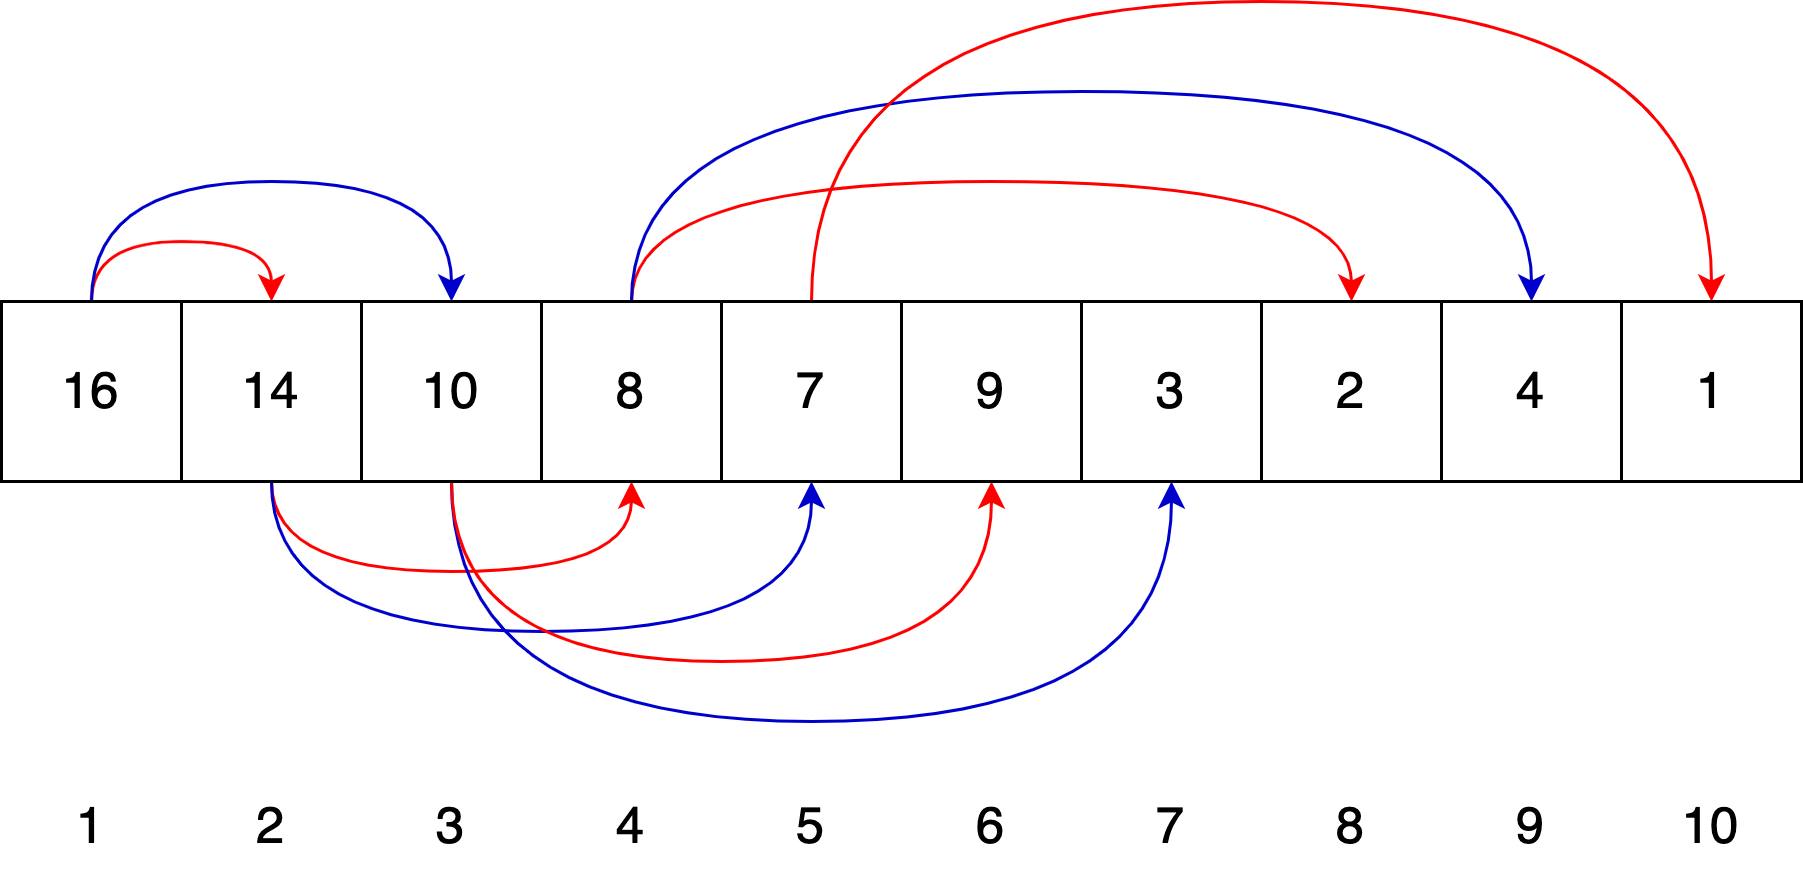
\includegraphics[scale=0.5]{img/binary-tree-in-array}
 \caption{完全二叉树到数组的映射} \label{fig:tree-array-map}
\end{figure}

\be
\begin{cases}
parent(i) & = \lfloor \dfrac{i}{2} \rfloor \\
left(i)   & = 2i \\
right(i)  & = 2i + 1 \\
\end{cases}
\ee

父节点和子树的访问可以通过位运算实现,见本章附录中的例子。

\subsection{堆调整}
\index{二叉堆!Heapify}

堆调整\footnote{Heapify,也译作堆化。}是维护堆性质的过程,使得堆顶元素为最小(或最大)。由于堆背后的数据模型是二叉树,我们可以利用树的递归特性,获得一个增强的堆性质:使得每棵子树的根节点都是最小(或最大)的。也就是说任何子树都代表一个子堆。简单起见,我们考虑小顶堆。对于用数组表示的二叉堆,任给数组下标$i$,我们检查$i$对应的所有子节点的值是否都不小于($\geq$)它。如果不满足则交换,使得父节点总保存最小值\cite{CLRS},并对以$i$为根的所有子树递归重复这个过程。如下算法定义了堆调整过程:

\begin{algorithmic}[1]
\Function{Heapify}{$A, i$}
  \State $n \gets |A|$
  \Loop
    \State $s \gets i$ \Comment{$s$指向最小}
    \State $l \gets$ \Call{Left}{$i$}, $r \gets$ \Call{Right}{$i$}
    \If{$l \leq n$ 且 $A[l] < A[i]$}
      \State $s \gets l$
    \EndIf
    \If{$r \leq n$ 且 $A[r] < A[s]$}
      \State $s \gets r$
    \EndIf
    \If{$s \neq i$}
      \State \textproc{Exchange} $A[i] \leftrightarrow A[s]$
      \State $i \gets s$
    \Else
      \State \Return
    \EndIf
  \EndLoop
\EndFunction
\end{algorithmic}

对于数组$A$和索引$i$,堆性质要求$A[i]$的子节点都不应比它小。否则,我选出最小的元素保存在$A[i]$,并将较大的元素交换至子树,然后自顶向下检查并调整堆,使得所有子树都满足堆性质。\textproc{Heapify}的时间复杂度为$O(\lg n)$,其中$n$是元素个数。这是因为算法中的循环次数和完全二叉树的高度成正比。图\ref{fig:heapify}描述了\textproc{Heapify}从索引2开始,按照小顶堆调整数组[1, 13, 7, 3, 10, 12, 14, 15, 9, 16]的步骤。数组最终变换为[1, 3, 7,9, 10, 12, 14, 15, 13, 16]。

\begin{figure}[htbp]
  \centering
  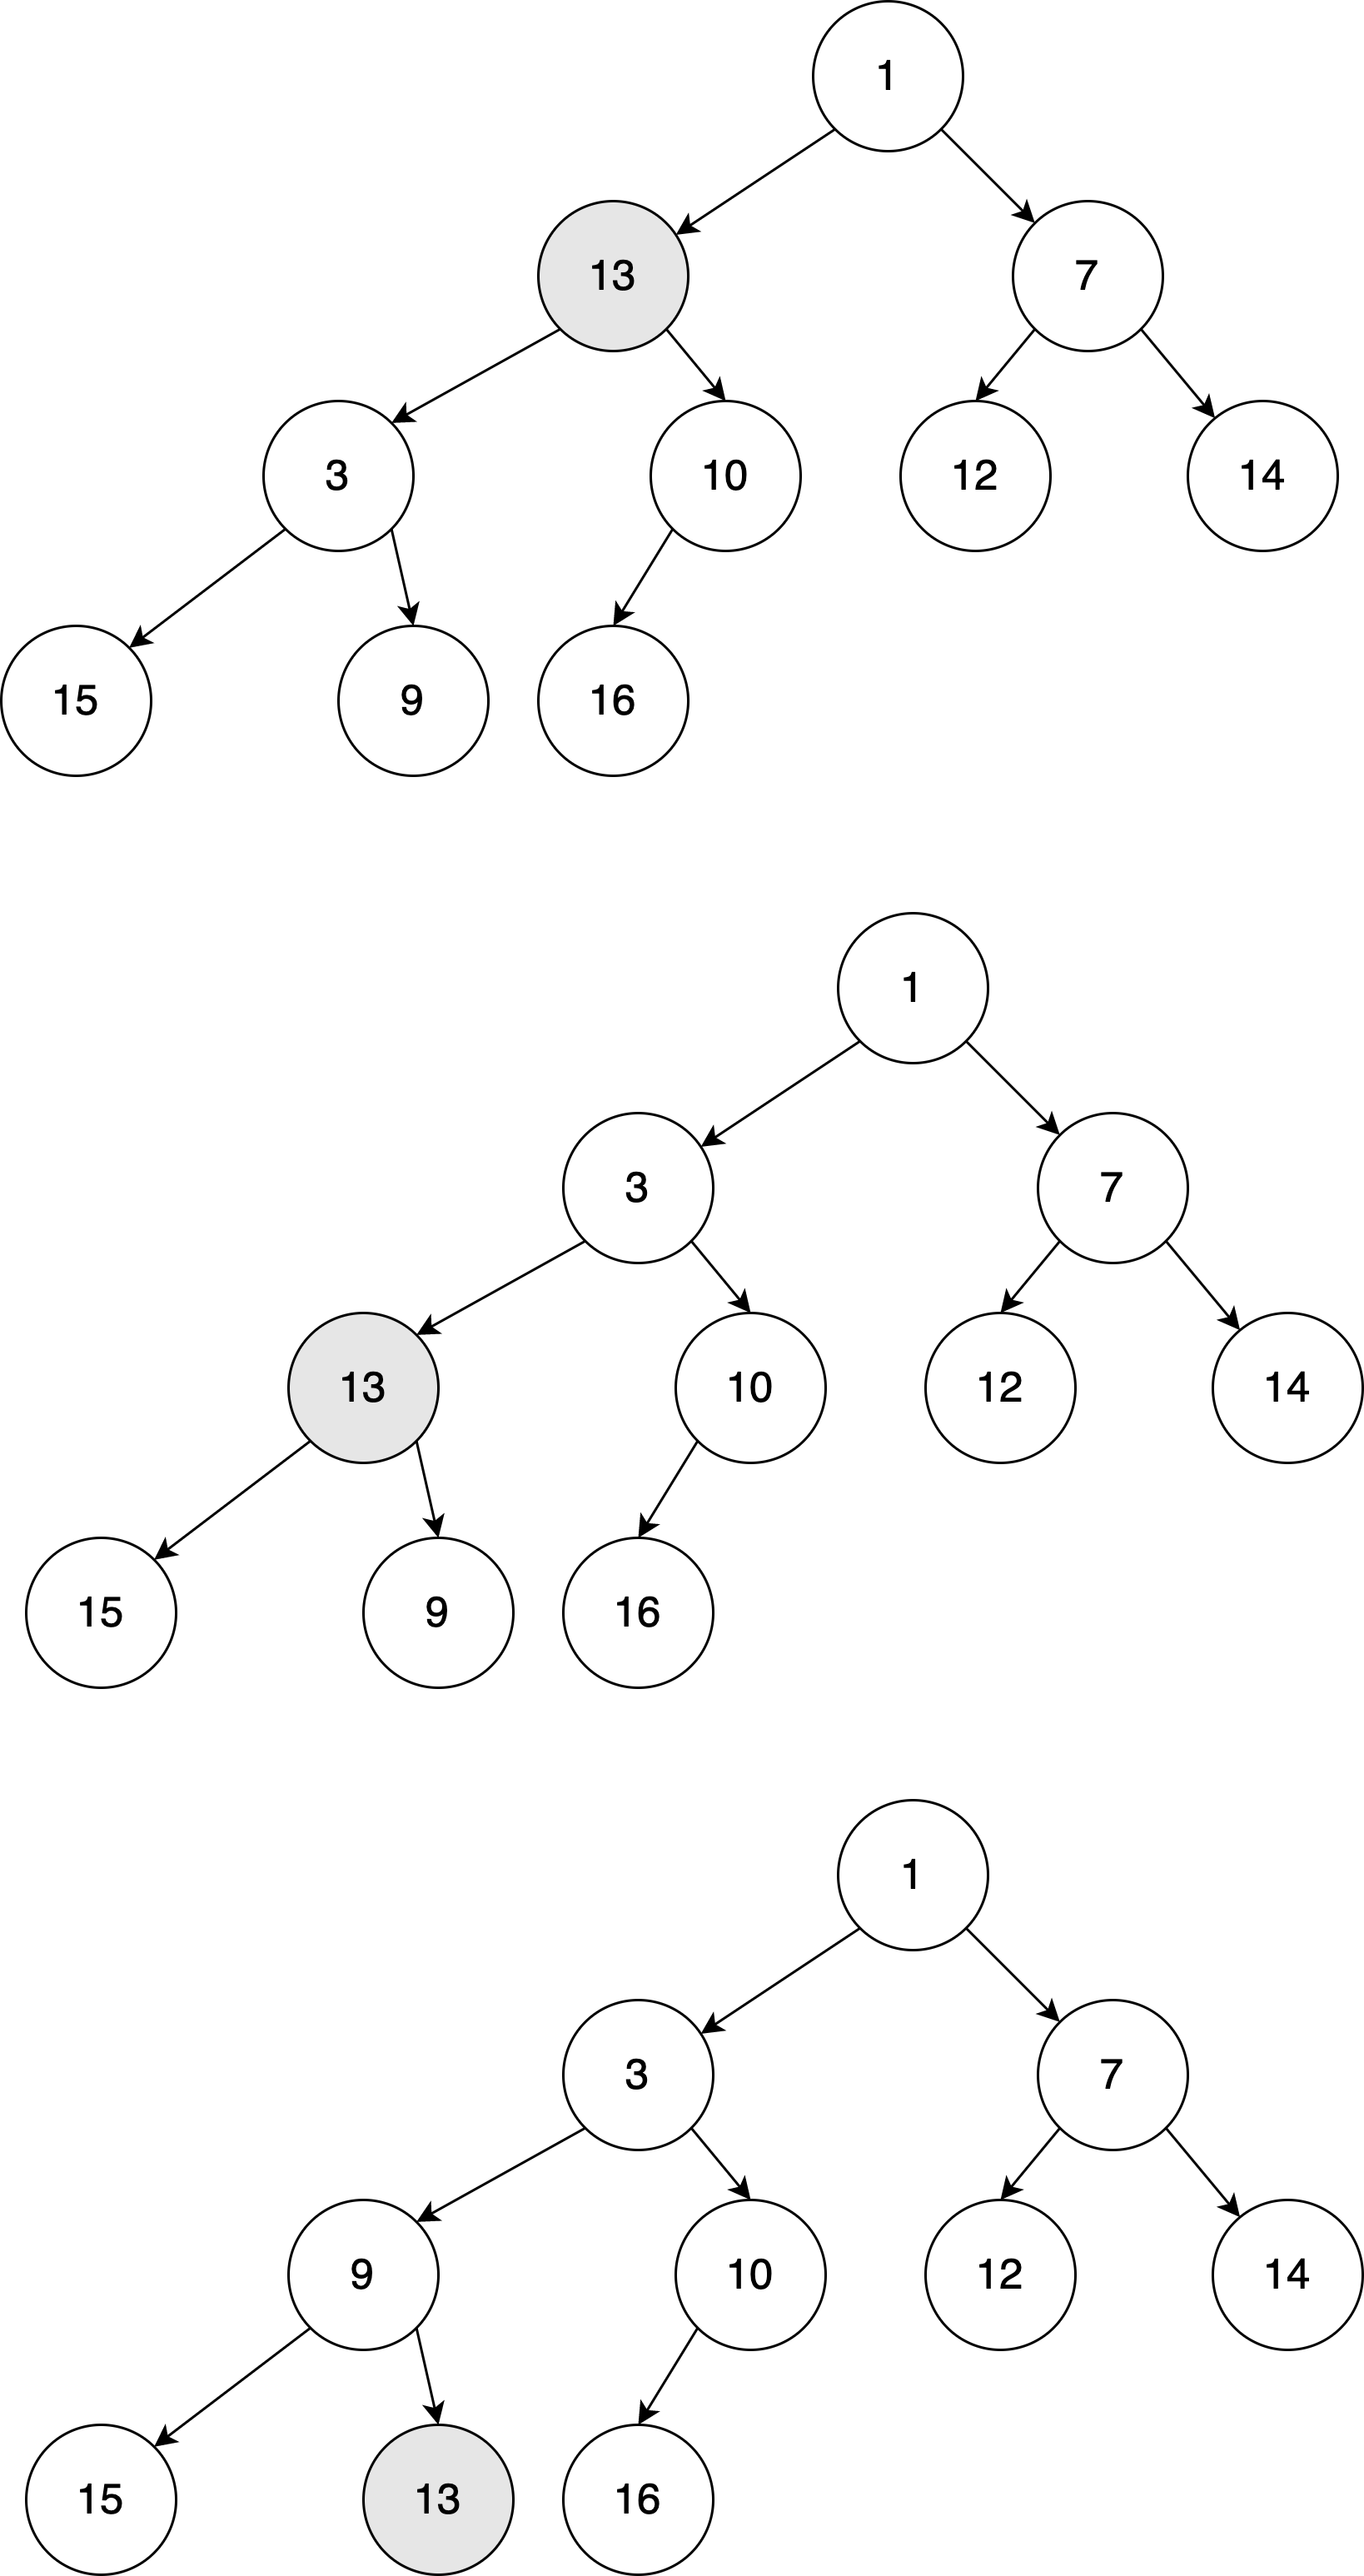
\includegraphics[scale=0.4]{img/heapify}
  \caption{堆调整。第一步:13、3、10中最小值为3,交换3 $\leftrightarrow$ 13;第二步:13、15、9中最小值为9,交换13 $\leftrightarrow$ 9;第三步:13为叶子节点,调整结束。}
  \label{fig:heapify}
\end{figure}

\subsection{构造堆}
\index{二叉堆!构造堆}

使用\textproc{Heapify},我们可以从任意数组构造出堆。观察完全二叉树各层的节点数目:$1, 2, 4, 8, ...$都是2的整数次幂,唯一例外是最后一层。由于树不一定满,最后一层最多含有$2^{p-1}$个节点,其中$p$是使得$2^p -1 \geq n$的最小整数,$n$是数组的长度。\textproc{Heapify}对叶子节点不起作用,因为叶子节点都已经满足堆性质了。我们跳过叶子节点,从第一个分支节点开始不断向上执行\textproc{Heapify}。显然第一个分支节点的索引不大于$\lfloor n/2 \rfloor$。我们可以设计出如下的堆构造算法:

\begin{algorithmic}[1]
\Function{Build-Heap}{$A$}
  \State $n \gets |A|$
  \For{$i \gets \lfloor n/2 \rfloor$ down to $1$}
    \State \Call{Heapify}{$A, i$}
  \EndFor
\EndFunction
\end{algorithmic}

虽然\textproc{Heapify}的复杂度为$O(\lg n)$,但是\textproc{Build-Heap}的复杂度不是$O(n \lg n)$,而是线性时间$O(n)$的。我们跳过了所有的叶子节点,最多有$1/4$的节点被比较并向下移动一次;最多有$1/8$的节点被比较并向下移动两次;最多有$1/16$的节点被比较并向下移动三次……总共比较和移动次数的上限为:

\be
S = n (\frac{1}{4} + 2 \frac{1}{8} + 3 \frac{1}{16} + ...)
\label{eq:build-heap-1}
\ee

将两侧都乘以2:

\be
2S = n (\frac{1}{2} + 2 \frac{1}{4} + 3 \frac{1}{8} + ...)
\label{eq:build-heap-2}
\ee

用式(\ref{eq:build-heap-2})减去式(\ref{eq:build-heap-1}),我们有:

\bea*{rcll}
2S - S & = & n [\dfrac{1}{2} + (2 \dfrac{1}{4} - \dfrac{1}{4}) + (3 \dfrac{1}{8} - 2 \dfrac{1}{8}) + ...] & \text{错开第一项两两相减} \\
     S & = & n [\dfrac{1}{2} + \dfrac{1}{4} + \dfrac{1}{8} + ...] & \text{等比级数和}\\
       & = & n
\eea*

图\ref{fig:build-heap-3}描述了从数组$[4, 1, 3, 2, 16, 9, 10, 14, 8, 7]$构造小顶堆的过程。黑色表示执行\textproc{Heapify}的目标节点;灰色表示进行交换的节点。

\begin{figure}[htbp]
  \centering
  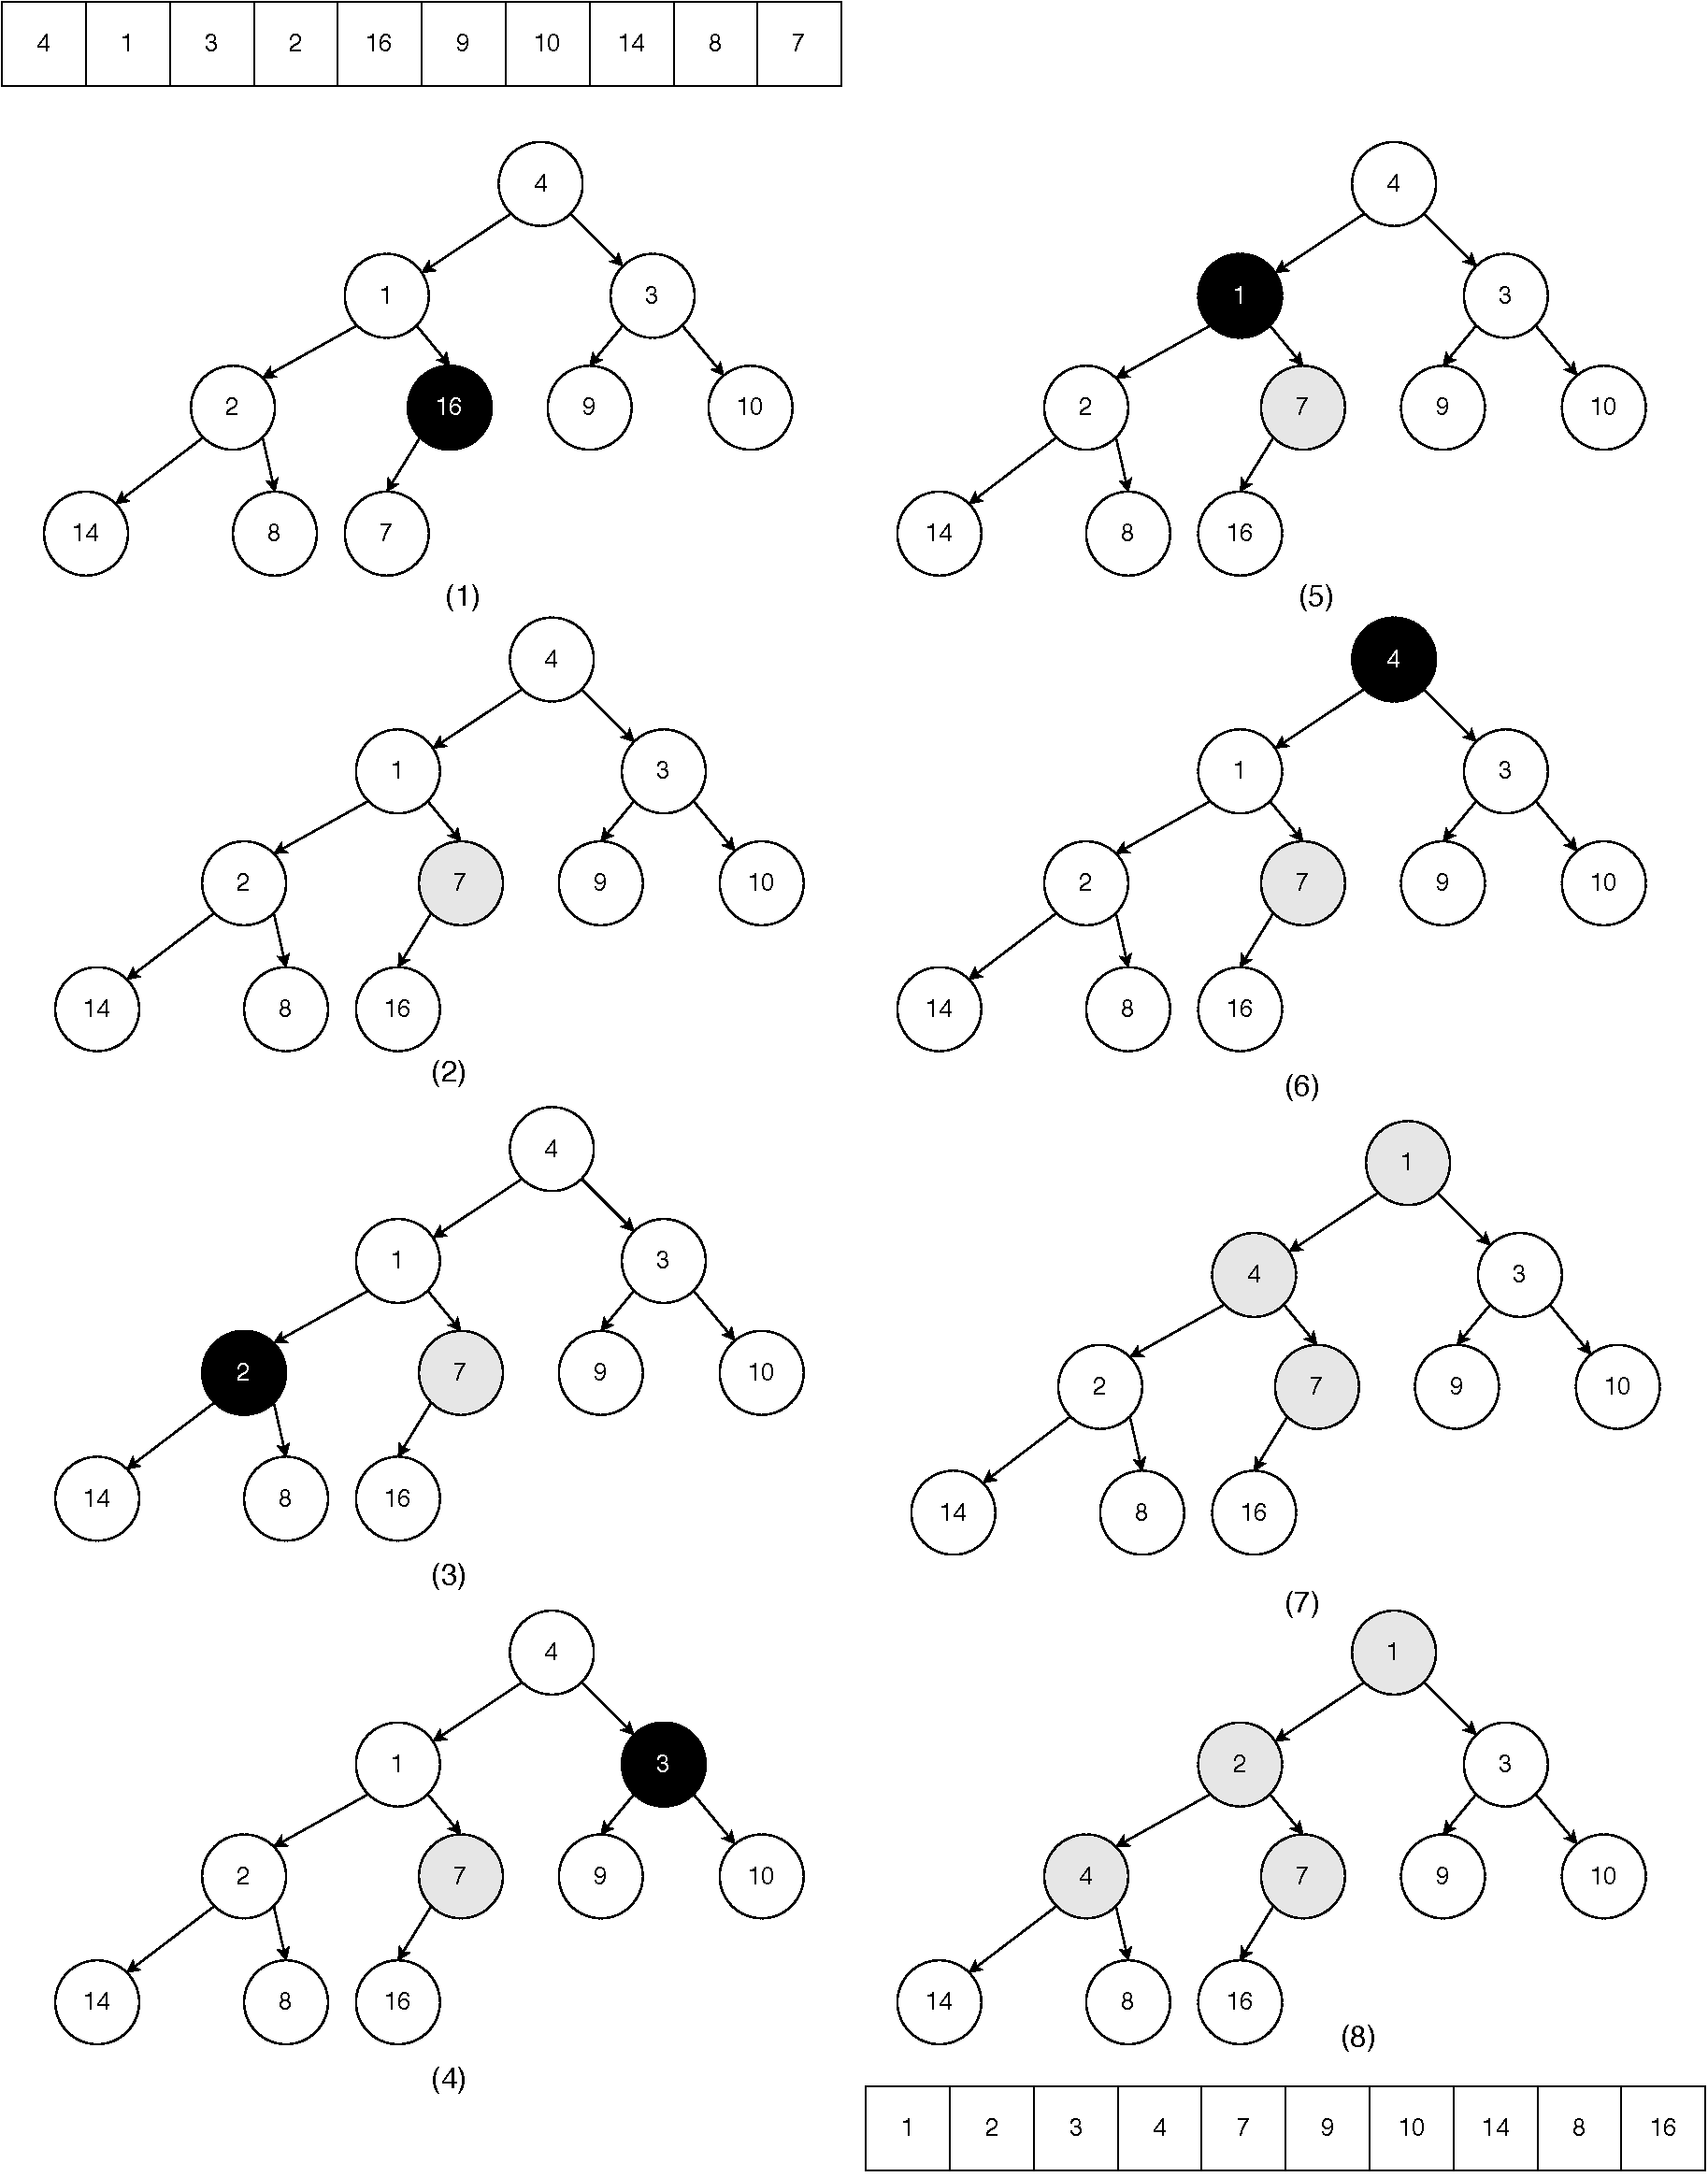
\includegraphics[scale=0.4]{img/build-heap}
  \caption{构造堆。(1)检查16,它大于子节点7;(2)交换16 $\leftrightarrow$ 7;(3)检查2,它比14,8都小;(4)检查3,它比9和10都小;(5)检查1,它比2和7都小;(6)检查4,1比4和3更小;(7)交换4 $\leftrightarrow$ 1;(8)交换4 $\leftrightarrow$ 2,结束。}
  \label{fig:build-heap-3}
\end{figure}

\subsection{堆的基本操作}

堆的基本操作包括获取顶部,弹出顶部,寻找最小(或最大)的前$k$个元素,减小小顶堆中某一元素(或增大大顶堆中某一元素),以及插入新元素。在用二叉树实现的堆中,根节点保存了顶部元素,它对应数组的第一个值:

\index{二叉堆!获取顶部元素}
\begin{algorithmic}[1]
\Function{Top}{$A$}
  \State \Return $A[1]$
\EndFunction
\end{algorithmic}

\subsubsection{弹出堆顶}
\index{二叉堆!弹出} \index{二叉堆!pop}

弹出堆顶后,数组剩余元素顺次向前移动。这相当于删除了二叉树的根节点,剩余部分不再保持一棵树状的结构。为了避免这种情况,我们可以将待移除的数组头部和末尾元素交换,然后将数组的长度减一,这相当于删除叶子节点而非根节点。最后再用\textproc{Heapify}恢复堆性质:

\begin{algorithmic}[1]
\Function{Pop}{$A$}
  \State $x \gets A [1], n \gets |A|$
  \State \textproc{Exchange} $A[1] \leftrightarrow A[n]$
  \State \Call{Remove}{$A, n$}
  \If{$A$ is not empty}
    \State \Call{Heapify}{$A$, 1}
  \EndIf
  \State \Return $x$
\EndFunction
\end{algorithmic}

从数组的末尾删除元素仅需常数时间,这样弹出操作的时间复杂度就取决于\textproc{Heapify},为$O(\lg n)$。

\subsubsection{Top-k}
\index{二叉堆!top-k}

连续使用pop,可以找出一组元素中的前$k$个最小(或最大):

\begin{algorithmic}[1]
\Function{Top-k}{$A, k$}
  \State $R \gets [\ ]$
  \State \Call{Build-Heap}{$A$}
  \Loop \ \textproc{Min}(k, |$A$|) times \Comment{$k$超出长度则截断}
    \State \textproc{Append}($R$, \Call{Pop}{$A$})
  \EndLoop
  \State \Return $R$
\EndFunction
\end{algorithmic}

\subsubsection{提升优先级}
\index{二叉堆!提升优先级}

堆的一个应用是实现带有优先级的任务调度,称为“优先级队列”。将若干带有优先级的任务放入堆中,每次从堆顶取出优先级最高的任务执行。为了尽早执行堆中的某个任务,可以提升它的优先级。对于小顶堆,这意味着减小某个元素的值,如图\ref{fig:decrease-key-2}所示。

\begin{figure}[htbp]
  \centering
  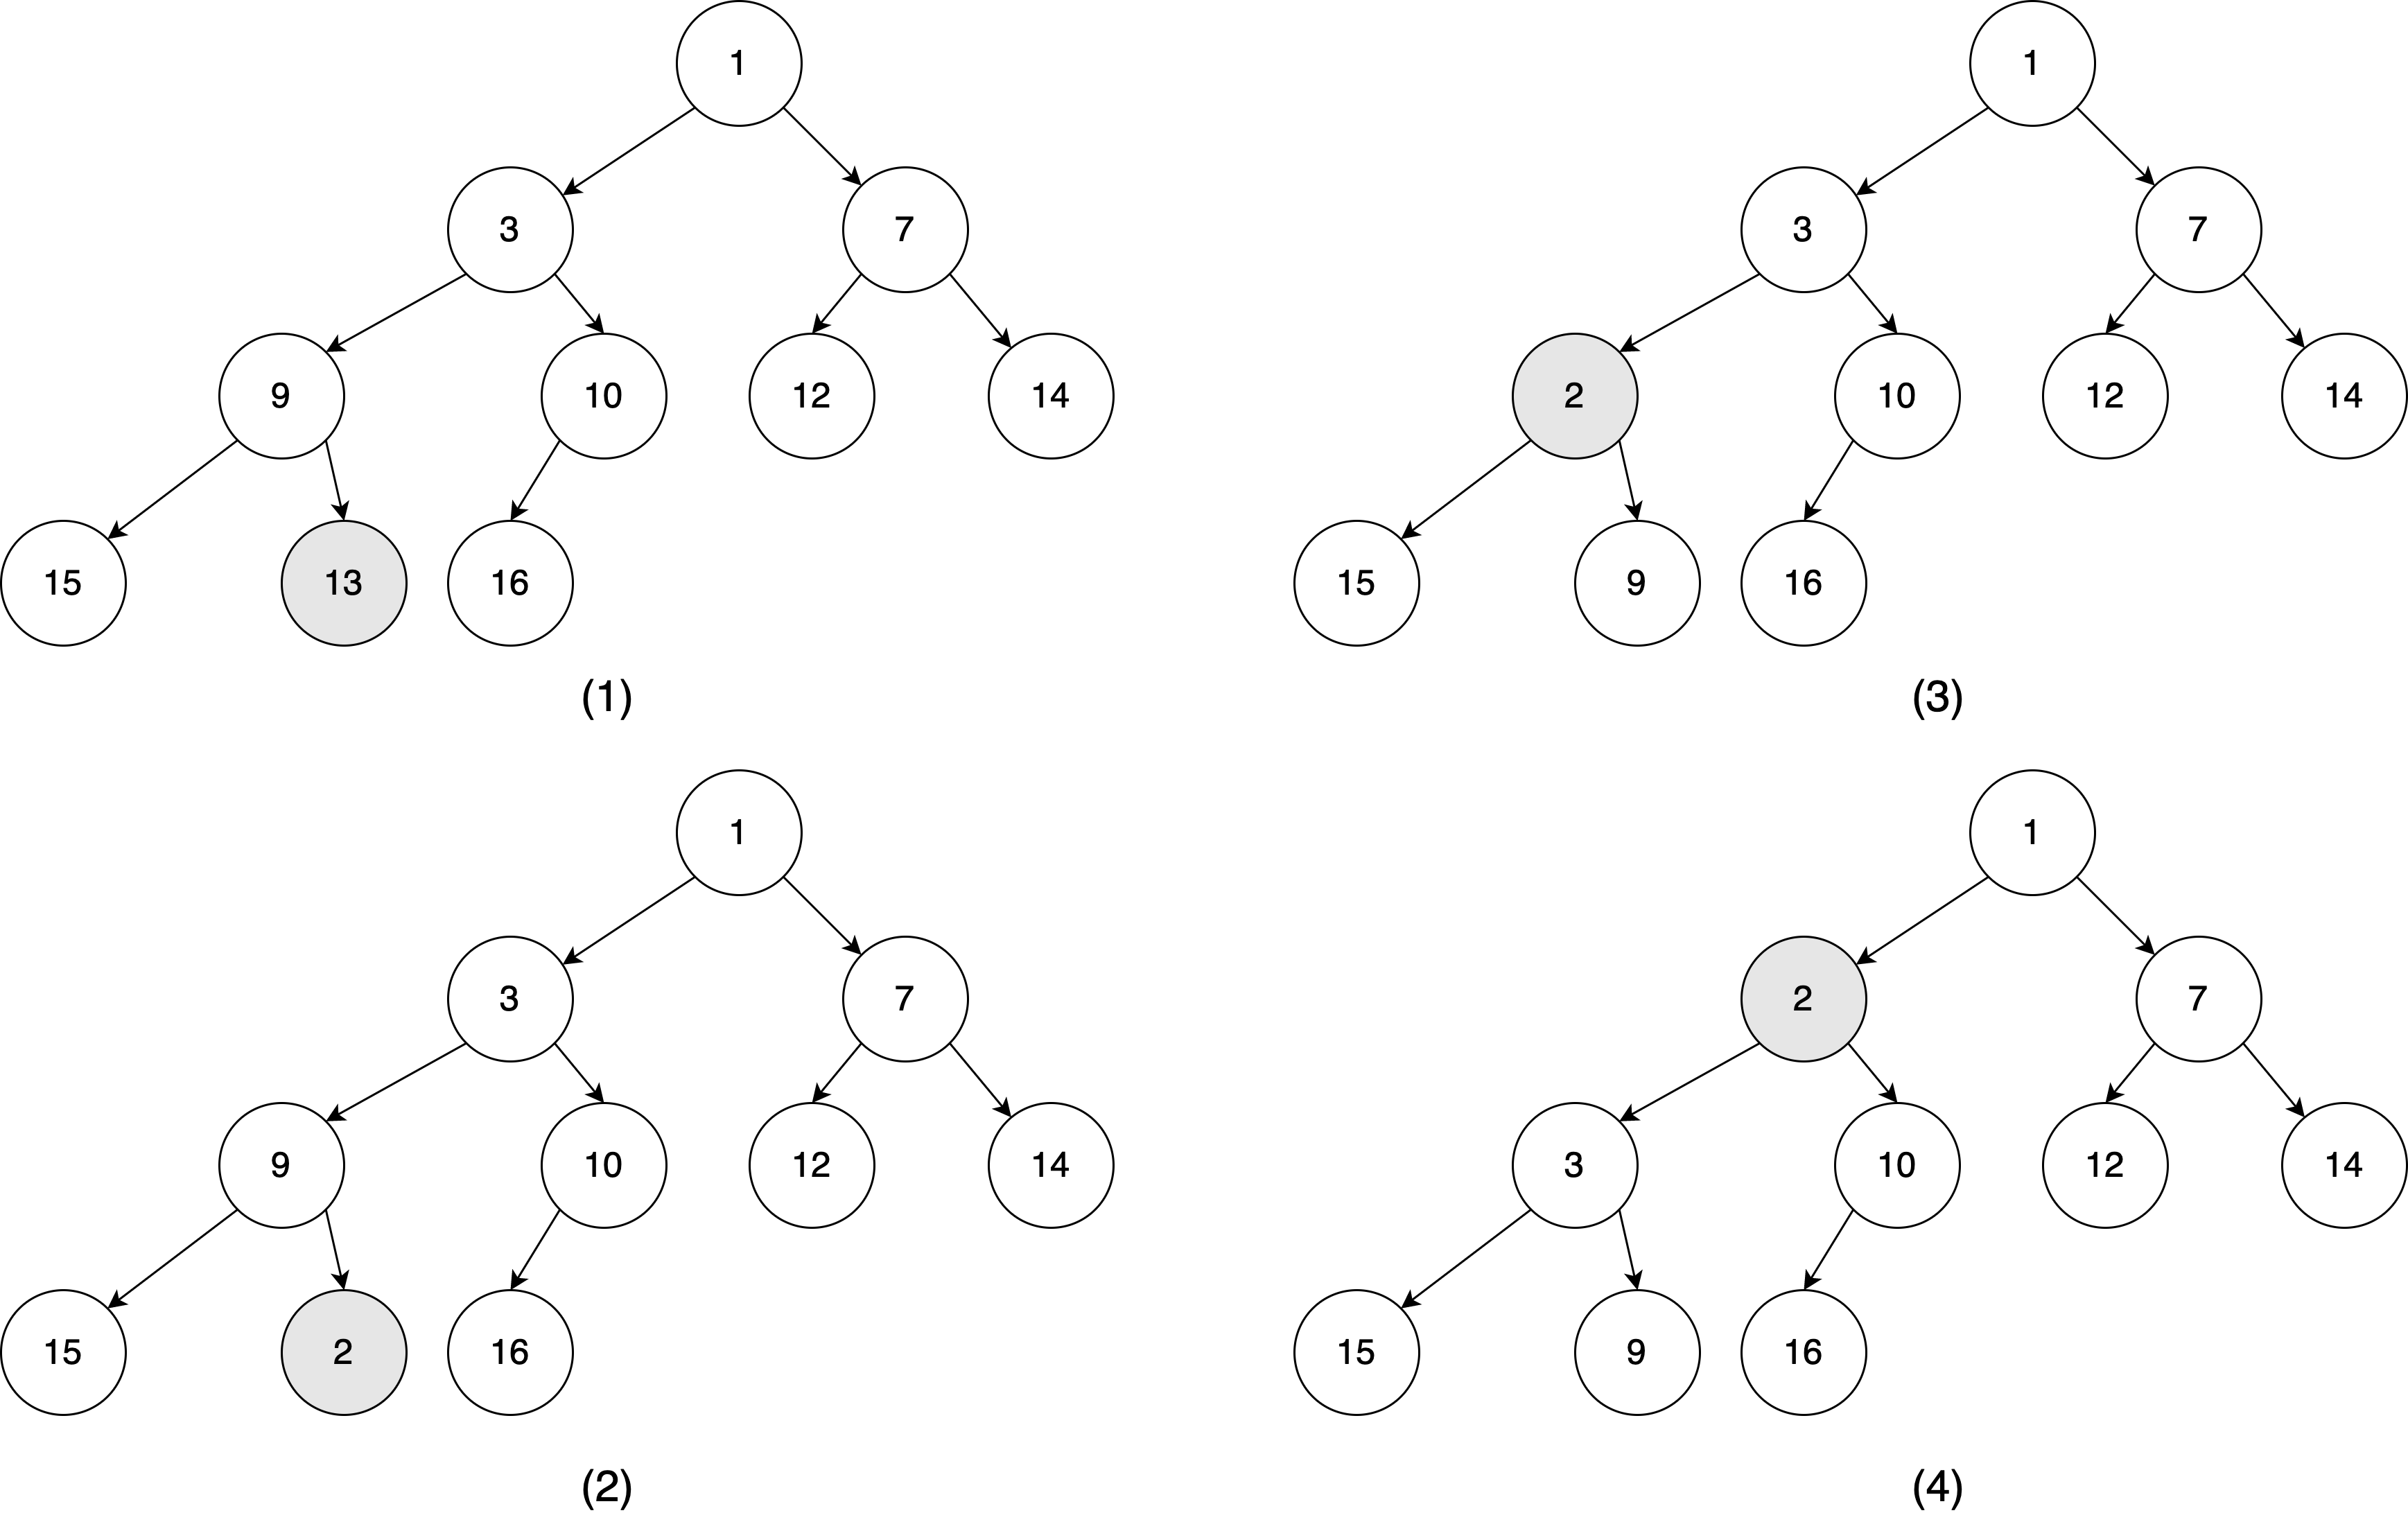
\includegraphics[scale=0.4]{img/decrease-key}
  \caption{将13减小为2。2先与9交换,然后再与3交换。}
  \label{fig:decrease-key-2}
\end{figure}

减小小顶堆中的某个元素时,可能会破坏堆性质。对于数组表示的二叉堆,令修改的元素索引为$i$,下面的算法自底向上恢复堆性质,其时间复杂度为$O(\lg n)$。

\begin{algorithmic}[1]
\Function{Heap-Fix}{$A, i$}
  \While{$i>1$ and $A[i] < A[$ \Call{Parent}{$i$} $]$}
    \State \textproc{Exchange} $A[i] \leftrightarrow A[$ \Call{Parent}{$i$} $]$
    \State $i \gets$  \Call{Parent}{$i$}
  \EndWhile
\EndFunction
\end{algorithmic}

\subsubsection{插入}
\index{二叉堆!插入(push)}

可以利用\textproc{Heap-Fix}来实现插入\cite{CLRS}。以小顶堆为例,先向数组末尾添加新元素$k$,再使用\textproc{Heap-Fix}调整:

\begin{algorithmic}[1]
\Function{Push}{$A, k$}
  \State \Call{Append}{$A, k$}
  \State \Call{Heap-Fix}{$A, |A|$}
\EndFunction
\end{algorithmic}

\subsection{堆排序}
\label{heap-sort} \index{堆排序}

可以利用堆实现排序。以小顶堆为例,从待排序元素构建一个堆,不断从堆顶获取最小元素,就获得了升序结果。若待排序的元素有$n$个,构建堆的时间复杂度是$O(n)$。由于弹出操作的复杂度为$O(\lg n)$,并且共执行了$n$次。因此总体时间复杂度为$O(n \lg n)$。由于我们使用了另外一个列表存放排序结果,因此空间复杂度为$O(n)$。

\begin{algorithmic}[1]
\Function{Heap-Sort}{$A$}
  \State $R \gets [\ ]$
  \State \Call{Build-Heap}{$A$}
  \While{$A \neq [\ ]$}
    \State \textproc{Append}($R$, \Call{Pop}{$A$})
  \EndWhile
  \State \Return $R$
\EndFunction
\end{algorithmic}

Robert. W. Floyd给出了另一种实现。思路是构建一个大顶堆。接下来,将堆顶的最大元素和数组末尾的元素交换,这样最大元素就存储到了排序后的正确位置。而原来在末尾的元素变成了新的堆顶。我们将堆的大小减一,然后执行\textproc{Heapify}恢复堆的性质。重复这一过程,直到堆中仅剩下一个元素。这一算法省去了额外的空间。

\begin{algorithmic}[1]
\Function{Heap-Sort}{$A$}
  \State \Call{Build-Max-Heap}{$A$}
  \State $n \gets |A|$
  \While{$n > 1$}
    \State \textproc{Exchange} $A[1] \leftrightarrow A[n]$
    \State $n \gets n - 1$
    \State \Call{Heapify}{$A[1...n], 1$}
  \EndWhile
\EndFunction
\end{algorithmic}

\begin{Exercise}
\Question{考虑另外一种实现原地堆排序的想法:第一步先从待排序数组构建一个最小堆$A$,此时,第一个元素$a_1$已经在正确的位置了。接下来,将剩余的元素$[a_2, a_3, ..., a_n]$当成一个新的堆,并从$a_2$开始执行\textproc{Heapify}。重复这一从左向右的步骤完成排序。这一方法正确么?
\begin{algorithmic}[1]
\Function{Heap-Sort}{$A$}
  \State \Call{Build-Heap}{$A$}
  \For{$i = 1$ to $n - 1$}
    \State \Call{Heapify}{$A[i ... n], 1$}
  \EndFor
\EndFunction
\end{algorithmic}
}

\Question{类似地,可以通过自左向右执行$k$遍\textproc{Heapify}来实现top-$k$算法么?
\begin{algorithmic}[1]
\Function{Top-K}{$A, k$}
  \State \Call{Build-Heap}{$A$}
  \State $n \gets |A|$
  \For {$i \gets 1$ to $min(k, n)$}
    \State \Call{Heapify}{$A[i ... n], 1$}
  \EndFor
\EndFunction
\end{algorithmic}
}
\end{Exercise}

\begin{Answer}
\Question{不正确。$[a_2, a_3, ..., a_n]$的结构不再是一个堆,仅对第一个元素使用\textproc{Heapify}是不够的,需要用\textproc{Build-Heap}重建堆。}
\Question{不可以,原因同上。}
\end{Answer}

\section{左偏堆和斜堆}
\label{ebheap}

考虑不用数组而用显式的二叉树实现堆。当弹出堆顶元素后,剩余部分是左右两棵子树,它们都是堆,如图\ref{fig:lvr}所示。我们如何将它们再次合并成一个堆呢?为保持堆性质,新的根节点必须是剩余元素中最小的。我们可以先给出两个特殊情况下的结果:

\begin{figure}[htbp]
  \centering
  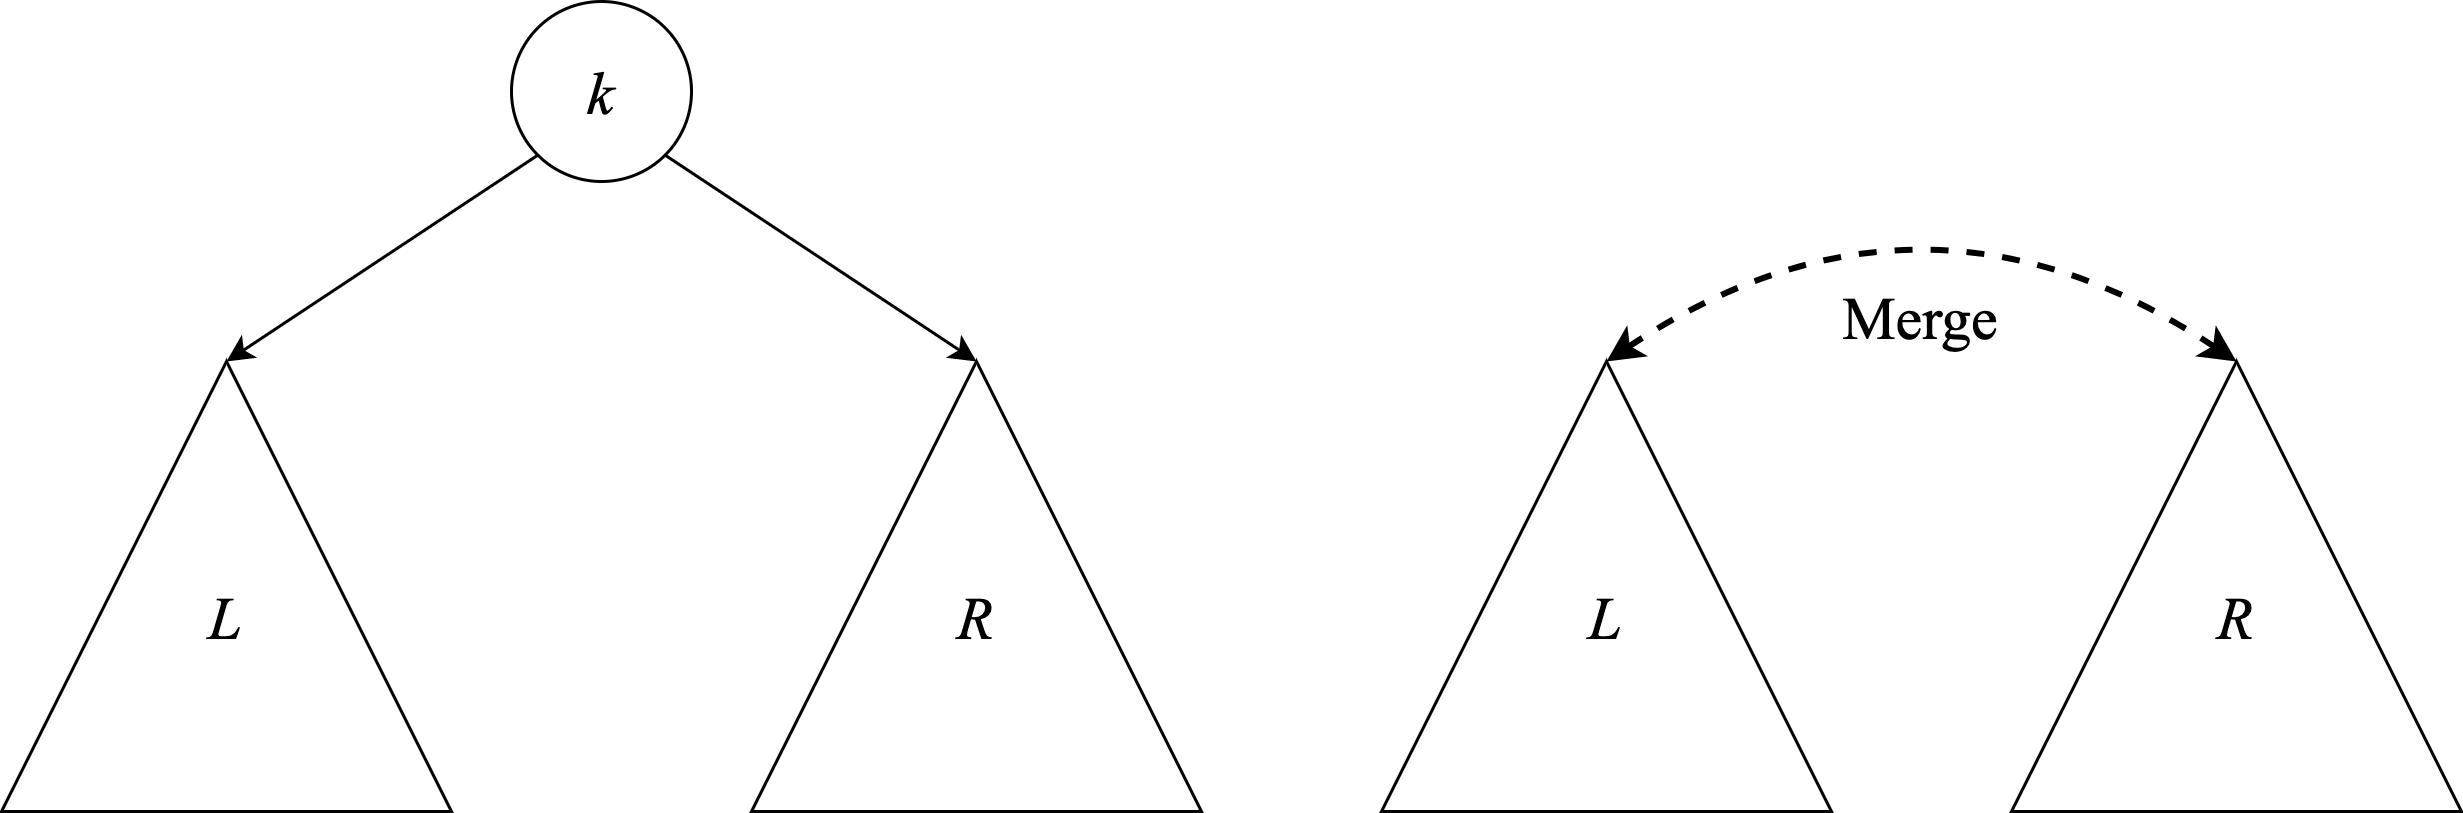
\includegraphics[scale=0.5]{img/lkr}
  \caption{弹出堆顶(删除根节点)后,合并左右子树形成一个堆。}
  \label{fig:lvr}
\end{figure}

\[
\begin{array}{rcl}
merge(\nil, R) & = & R \\
merge(L, \nil) & = & L \\
merge(L, R) & = & ? \\
\end{array}
\]

左右子树都不为空时,由于它们也都是堆,各自的根节点都保存了最小的元素。我们可以比较两棵子树的根,选择较小的一个作为合并后的根。令$L = (A, x, B)$、$R = (A', y, B')$,其中$A$、$A'$、$B$、$B'$都是子树。如果$x < y$,$x$就是新的根。我们可以保留$A$,然后递归地合并$B$和$R$;或者保留$B$,递归地合并$A$和$R$。新的堆可以为$(merge(A, R), x, B)$或$(A, x, merge(B, R))$之一。两个都可以,为了简单,我们可以总选择右子树进行合并。这样的堆称为\textbf{左偏堆}({\em Leftist} heap)。

\subsection{左偏堆}
\index{左偏堆} \index{左偏堆!秩} \index{左偏堆!S-值}

使用左偏树实现的堆称为左偏堆。左偏树最早由C. A. Crane于1972年引入\cite{wiki-leftist-tree}。树中每个节点都定义了一个秩,也称作$S$值。节点的秩是到最近的NIL节点的距离。而NIL节点的秩等于0。如图\ref{fig:rank}所示,距离根节点4最近的叶子节点为8,所以根节点的秩为2。节点6和8都是叶子,它们的秩为1。虽然节点5的左子树不为空,但是它的右子树为空,因此秩等于1。使用秩,我们可以定义合并策略如下,记左右子树的秩分别为$r_l$、$r_r$:

\begin{figure}[htbp]
  \centering
  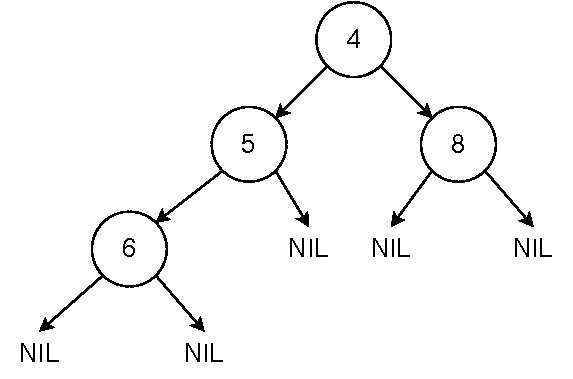
\includegraphics[scale=0.45]{img/rank}
  \caption{$rank(4) = 2$、$rank(6) = rank(8) = rank(5) = 1$}
  \label{fig:rank}
\end{figure}

\begin{enumerate}
\item 总是合并右子树;
\item 若$r_l < r_r$,就交换左右子树。
\end{enumerate}

我们称这样的合并策略为“左偏性质”。概括来说,在一棵左偏树中,到某个NIL的最短距离总在右侧。左偏树总是趋向不平衡,但是它可以维护一条重要的性质:

\begin{theorem}
若一棵左偏树$T$包含$n$个节点,从根节点到达最右侧NIL的路径上最多含有$\lfloor \log (n + 1) \rfloor$个节点。
\end{theorem}

我们这里省略了证明\cite{brono-book}, \cite{TAOCP-bheap}。根据此定理,沿着这一路径进行操作的算法,都可以保证$O(\lg n)$的复杂度。我们可以在二叉树的基础上增加一个秩来定义左偏树。记非空的左偏树为$(r, L, k, R)$,分别表示秩、左子树、元素值、右子树:

\lstset{frame = single}
\begin{Haskell}
data LHeap a = E -- 空
             | Node Int (LHeap a) a (LHeap a)
\end{Haskell}

定义$rank$函数返回节点的秩。

\be
\begin{array}{rcl}
rank\ \nil & = & 0 \\
rank\ (r, L, k, R) & = & r \\
\end{array}
\ee

\subsubsection{合并}
\index{左偏堆!合并}

为了实现合并,我们定义$make$函数比较左右子树的秩,并交换子树保持左偏性质。

\be
make(A, k, B) = \begin{cases}
  rank(A) < rank(B) : & (rank(A) + 1, B, k, A) \\
  \text{否则}: & (rank(B) + 1, A, k, B) \\
  \end{cases}
\ee

传入两棵子树$A$、$B$和元素$k$。若$A$的秩较小,则用$B$作为左子树、$A$作为右子树。新节点的秩为$rank(A) + 1$;否则,若$B$的秩较小,就用$A$作为左子树,$B$作为右子树。新节点的秩为$rank(B) + 1$。给定两个左偏堆$H_1$和$H_2$,它们不空时分别记为$(r_1, L_1, K_1, R_1)$、$(r_2, L_2, k_2, R_2)$,下面的函数定义了合并操作:

\be
\begin{array}{rcl}
  \textit{merge}\ \nil\ H_2 & = & H_2 \\
  \textit{merge}\ H_1\ \nil & = & H_1 \\
  \textit{merge}\ H_1\ H_2 & = & \begin{cases}
  k_1 < k_2 : & make(L_1, k_1, \textit{merge}\ R_1\ H_2)  \\
  \text{否则}: & make(L_2, k_2, \textit{merge}\ H_1\ R_2) \\
  \end{cases}
\end{array}
\ee

$merge$总在右子树上进行递归,左偏性质得以保持。这样就保证了算法的复杂度为$O(\lg n)$。回顾上节,使用数组实现的堆在大多数情况下性能很好,并且和计算机的高速缓存技术配合良好。但是合并操作的时间复杂度却为线性时间$O(n)$。我们需要将两个数组连接起来,然后重新构建堆\cite{NIST}。

\begin{algorithmic}[1]
\Function{Merge-Heap}{$A, B$}
  \State $C \gets$ \Call{Concat}{$A, B$}
  \State \Call{Build-Heap}{$C$}
\EndFunction
\end{algorithmic}

使用$merge$函数,可以实现基本的堆操作。

\subsubsection{弹出顶部}
\index{左偏堆!top} \index{左偏堆!pop} \index{左偏堆!弹出}

我们可以在$O(1)$时间内获取根节点中的堆顶元素(设若树不为空):

\be
top\ (r, L, k, R) = k
\ee

弹出顶部后,我们将左右子树合并为一个新堆。弹出的时间复杂度和$merge$相同,也是$O(\lg n)$。

\be
pop\ (r, L, k, R) = merge\ L\ R
\ee

\subsubsection{插入}
\index{左偏树!插入}

插入新元素$k$时,可以从$k$构造出只有一个叶子节点的树,然后将它和合并到待插入的树中:

\be
insert\ k\ H = merge\ (1, \nil, k, \nil)\ H
\ee

或写成克里化的形式$insert\ k\ = merge\ (1, \nil, k, \nil)$。这样插入的时间复杂度也和合并相同,为$O(\lg n)$。我们可以将一个列表中的元素依次插入,从列表构造左偏堆。图\ref{fig:leftist-tree}给出了一个构造左偏堆的例子。

\be
build\ L = fold_r\ insert\ \nil\ L
\ee

对应的克里化形式为:$build = fold_r\ insert\ \nil$

\begin{figure}[htbp]
  \centering
  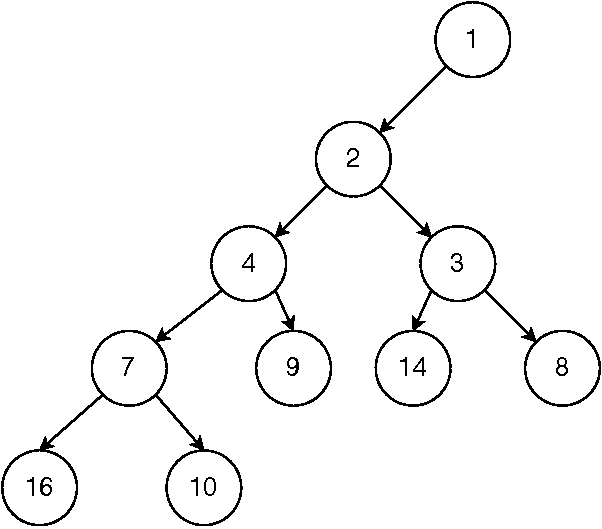
\includegraphics[scale=0.5]{img/leftist-tree}
  \caption{从列表$[9, 4, 16, 7, 10, 2, 14, 3, 8, 1]$构造左偏堆}
  \label{fig:leftist-tree}
\end{figure}

\subsubsection{堆排序}
\index{左偏树!堆排序}

给定一个序列,将它转换成一个左偏堆,然后不断取出堆顶的最小元素就可以实现排序:

\be
sort = heapSort \circ build
\ee

其中:
\be
\begin{array}{rcl}
heapSort\ [\ ] & = & [\ ] \\
heapSort\ H & = & (top\ H) : (heapSort\ (pop\ H)) \\
\end{array}
\ee

弹出需要对数时间,并且被调用了$n$次,因此排序的总复杂度为$O(n \lg n)$。

\subsection{斜堆}
\label{skew-heap} \index{斜堆}

左偏堆在某些情况下会产生不平衡的结构,如图\ref{fig:unbalanced-leftist-tree}所示。斜堆(skew heap)是一种自调整堆,它简化了左偏堆的实现并提高了平衡性\cite{wiki-skew-heap}、\cite{self-adjusting-heaps}。构造左偏堆时,若左侧的秩小于右侧,则交换左右子树。但是这一策略不能很好处理某一分支含有一个NIL子节点的情况:不管树有多大,它的秩总为1。斜堆简化了合并策略:每次都交换左右子树。

\begin{figure}[htbp]
  \centering
  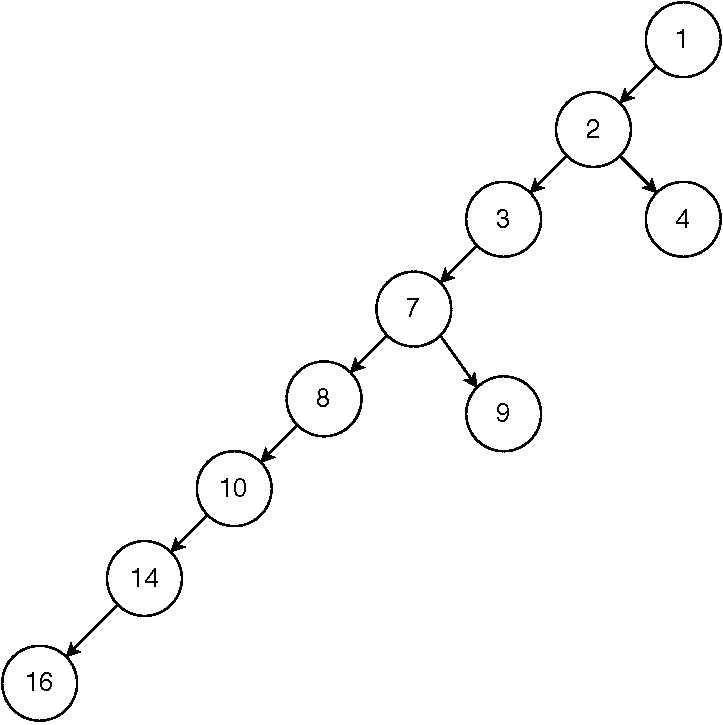
\includegraphics[scale=0.45]{img/unbalanced-leftist-tree}
  \caption{从序列$[16, 14, 10, 8, 7, 9, 3, 2, 4, 1]$构造的左偏堆}
  \label{fig:unbalanced-leftist-tree}
\end{figure}

斜堆是由斜树(skew tree)实现的堆。斜树是一种特殊的二叉树。最小的元素保存在根节点,每棵子树也都是一棵斜树。它不保存秩,可以直接复用二叉树的定义。树或者为空,或记为$(L, k, R)$。

\begin{Haskell}
data SHeap a = E -- 空
             | Node (SHeap a) a (SHeap a)
\end{Haskell}

\subsubsection{合并}
\index{斜堆!合并} \index{斜堆!插入} \index{斜堆!top} \index{斜堆!pop} \index{斜堆!弹出}

当合并两棵非空斜树时,先比较根节点,选择较小的作为新的根。然后把含有较大元素的树合并到某一子树上。最后再把左右子树交换。令两棵非空子树为:$H_1 = (L_1, k_1, R_1)$、$H_2 =(L_2, k_2, R_2)$。若$k_1 < k_2$,选择$k_1$作为新的根。我们既可以将$H_2$和$L_1$合并,也可以将$H_2$和$R_1$合并。不失一般性,我们合并到$R_1$上。然后交换左右子树,最后的结果为$(merge(R_1, H_2), k_1, L_1)$。

\be
\begin{array}{rcl}
merge\ \nil\ H_2 & = & H_2 \\
merge\ H_1\ \nil & = & H_1 \\
merge\ H_1\ H_2\ & = & \begin{cases}
  k_1 < k_2: & (merge(R_1, H_2), k_1, L_1) \\
  \text{否则}: & (merge(H_1, R_2), k_2, L_2) \\
\end{cases}
\end{array}
\ee

其他的操作,包括插入,获取和弹出顶部都和左偏树一样通过合并来实现。即使用斜堆处理已序序列,结果仍然是一棵较平衡的二叉树,如图\ref{fig:skew-tree}所示。

\begin{figure}[htbp]
  \centering
  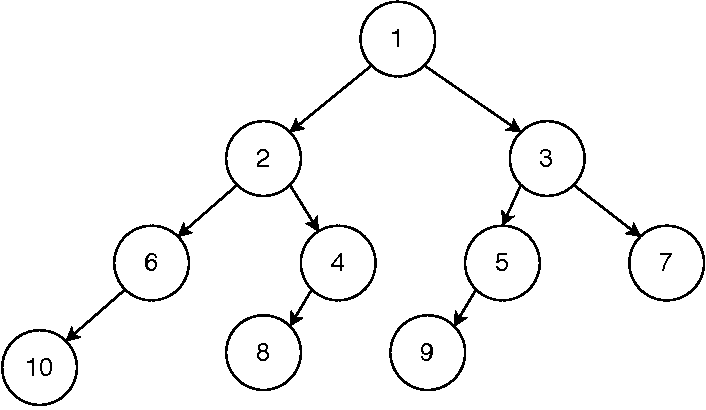
\includegraphics[scale=0.5]{img/skew-tree}
  \caption{用已序序列$[1, 2, ..., 10]$构造的斜树}
  \label{fig:skew-tree}
\end{figure}

\section{伸展堆}
\label{splayheap} \index{伸展堆}

左偏堆和斜堆是直接用二叉树实现的堆。如果将二叉树换成二叉搜索树,则最小(或最大)元素就不再位于根节点。我们需要$O(\lg n)$时间来获取最小(或最大)元素。如果二叉搜索树不平衡,性能会下降。最坏情况下会退化为$O(n)$。尽管可以用红黑树来保持平衡,伸展树提供了一种轻量级的实现方法,使得树不断趋向平衡。伸展树采用类似于缓存的策略,它不断将正在访问的节点向根旋转,这样再次访问的时候就可以更快。我们将这样的操作称为“伸展(splay)”。对于不平衡的二叉搜索树,经过若干次伸展后,树会变得逐渐平衡。大多数伸展树操作的均摊性能是$O(\lg n)$的。Daniel Dominic Sleator和Robert Endre Tarjan在1985年最早引入了伸展树\cite{wiki-splay-tree}\cite{self-adjusting-trees}。

\subsection{伸展操作}
\index{伸展堆!splay}

有两种方法可以实现伸展操作。第一种利用模式匹配,但需要处理较多的情况;第二种具备统一的形式,但是实现较为复杂。记正在访问的节点元素为$x$,它的父节点元素为$p$,如果存在祖父节点,其元素记为$g$。伸展操作分为三个步骤,每个步骤有两个对称的情况,我们以每步中的一种情况举例说明,如图\ref{fig:splay}所示。

\begin{enumerate}
\item zig-zig步骤,$x$和$p$都是左子树或者$x$和$p$都是右子树。我们通过两次旋转,将$x$变成根节点。

\item zig-zag步骤,$x$和$p$一棵是左子树另一棵是右子树。经过旋转,$x$变成根节点,$p$和$g$变成了兄弟节点。

\item zig步骤,这种情况下,$p$是根节点,经过旋转,$x$变成了根节点。这是伸展操作的最后一步。
\end{enumerate}

\begin{figure}[htbp]
  \centering
  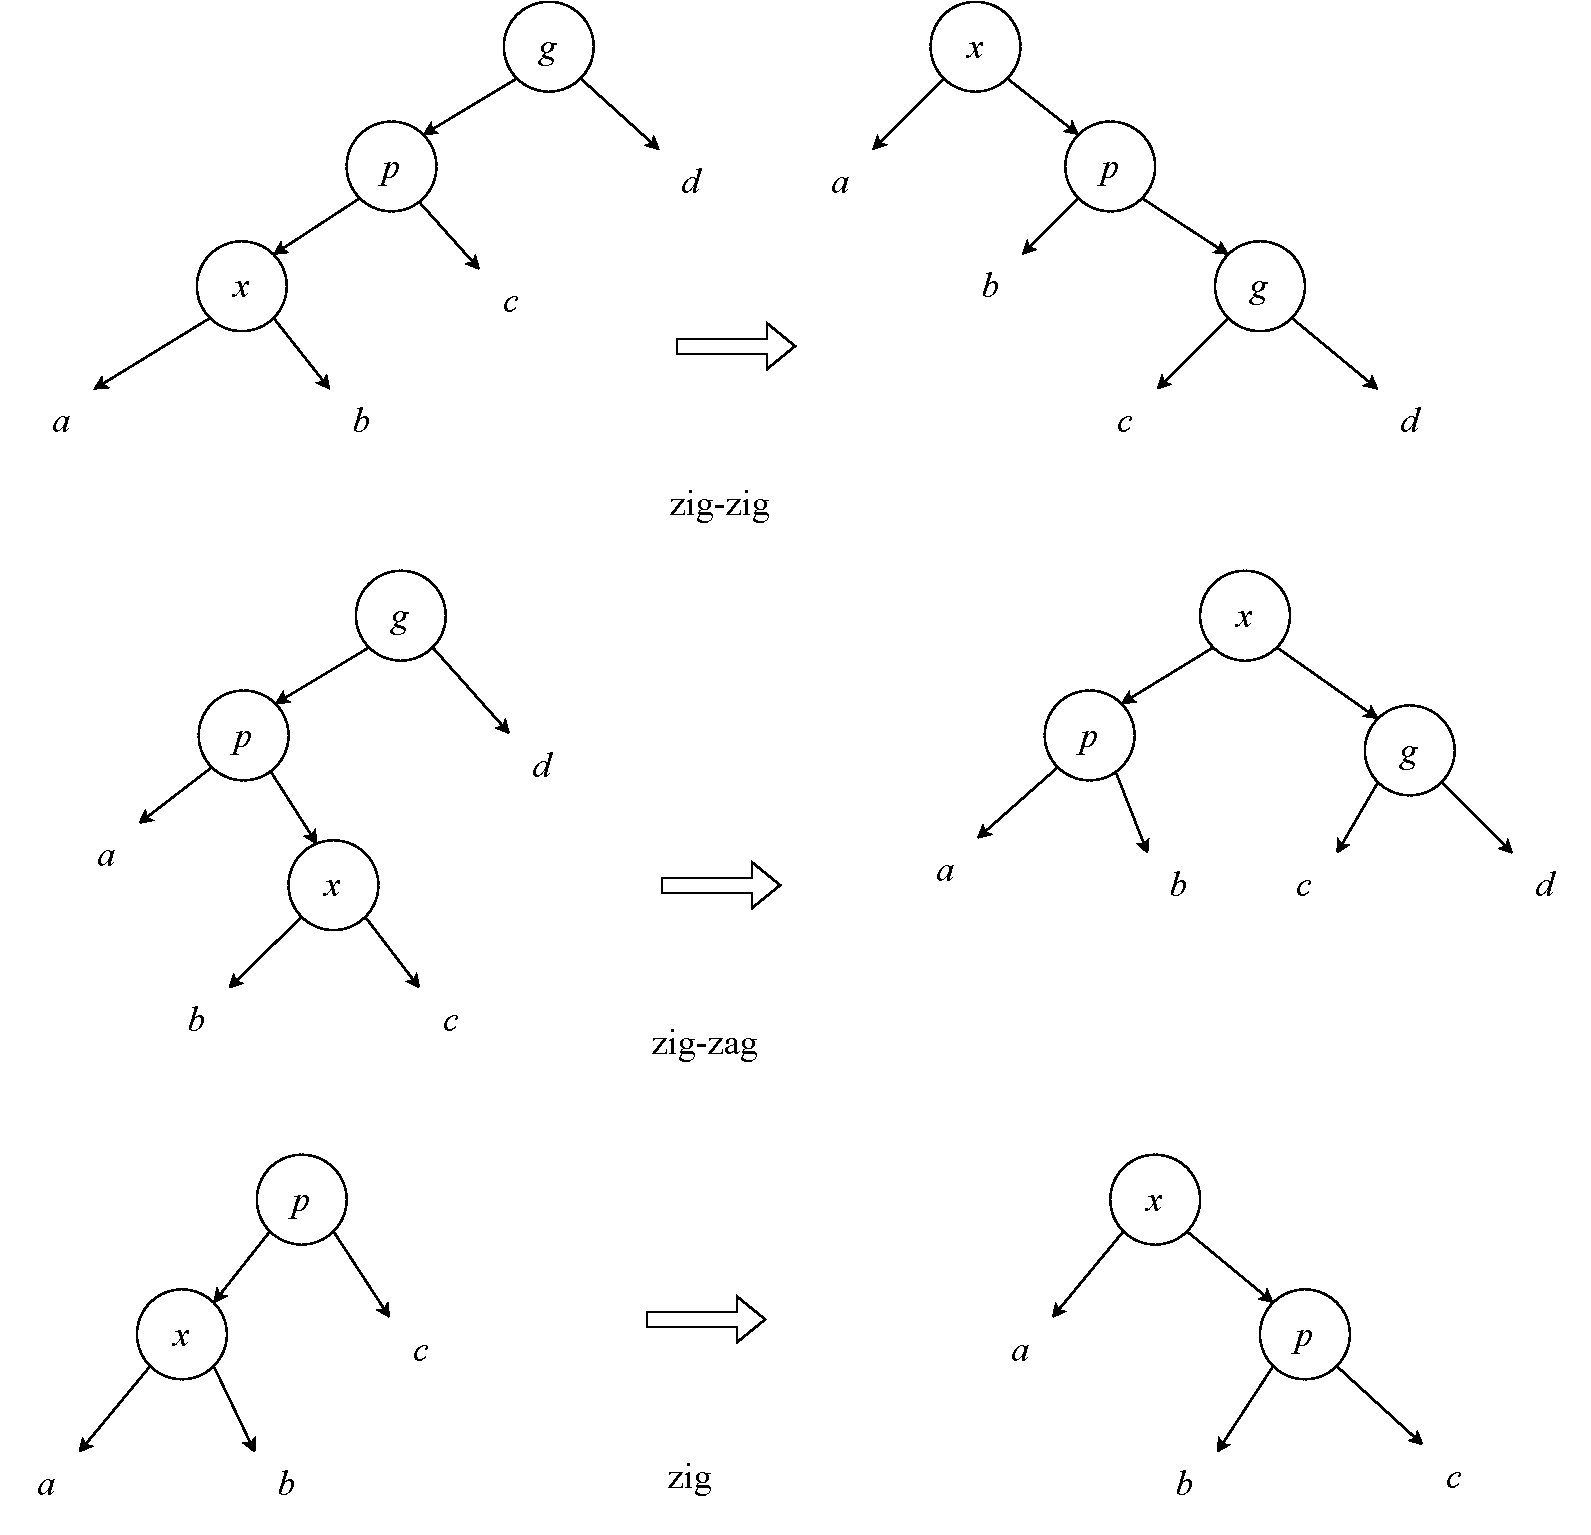
\includegraphics[scale=0.45]{img/splay}
  \caption{zig-zig: $x$和$p$都是左子树或都是右子树,$x$成为根节点。zig-zag: $x$和$p$一棵是左子树另一棵是右子树,$x$成为根节点,$p$和$g$变成了兄弟节点。zig: $p$是根节点,旋转后$x$变为根节点。}
  \label{fig:splay}
\end{figure}

共有6种不同的情况。记非空二叉树为$T=(L, k, R)$,当访问树中的元素$y$时,伸展操作定义如下:

\be
\begin{array}{rcll}
splay\ (((a, x, b), p, c), g, d)\ y & = & \begin{cases}
    x = y: & (a, x, (b, p, (c, g, d))) \\
    \text{否则}: & T \\
  \end{cases} & \text{zig-zig} \\
splay\ (a, g, (b, p, (c, x, d)))\ y & = & \begin{cases}
    x = y: & (((a, g, b), p, c), x, d) \\
    \text{否则}: & T \\
  \end{cases} & \text{zig-zig对称} \\
splay\ (a, p, (b, x, c), g, d)\ y & = & \begin{cases}
    x = y: & ((a, p, b), x, (c, g, d)) \\
    \text{否则}: & T \\
  \end{cases} & \text{zig-zag} \\
splay\ (a, g, ((b, x, c), p, d))\ y & = & \begin{cases}
    x = y: & ((a, g, b), x, (c, p, d)) \\
    \text{否则}: & T \\
  \end{cases} & \text{zig-zag对称} \\
splay\ ((a, x, b), p, c)\ y & = & \begin{cases}
    x = y: & (a, x, (b, p, c)) \\
    \text{否则}: & T \\
  \end{cases} & \text{zig} \\
splay\ (a, p, (b, x, c))\ y & = & \begin{cases}
    x = y: & ((a, p, b), x, c) \\
    \text{否则}: & T \\
  \end{cases} & \text{zig对称} \\
splay\ T\ y & = & T & \text{其它} \\
\end{array}
\ee

前两条子式处理zig-zig情况;接下来的两条子式处理zig-zag情况;最后两条子式处理zig情况。其他情况下,树都保持不变。每次插入新元素时,我们就执行伸展操作来调整树的平衡性。如果树为空,结果为一个叶子节点;否则我们比较待插入的元素和根节点,如果待插入的元素较小,就将其递归插入左子树,然后执行伸展操作;否则插入右子树,再执行伸展操作。

\be
\begin{array}{rcl}
insert\ \nil\ y & = & (\nil, y, \nil) \\
insert\ (L, x, R)\ y & = & \begin{cases}
  y < x: & splay\ ((insert\ L\ y), x, R)\ y  \\
  \text{否则}: & splay\ (L, x, (insert\ R\ y))\ y \\
\end{cases}
\end{array}
\ee

\begin{figure}[htbp]
  \centering
  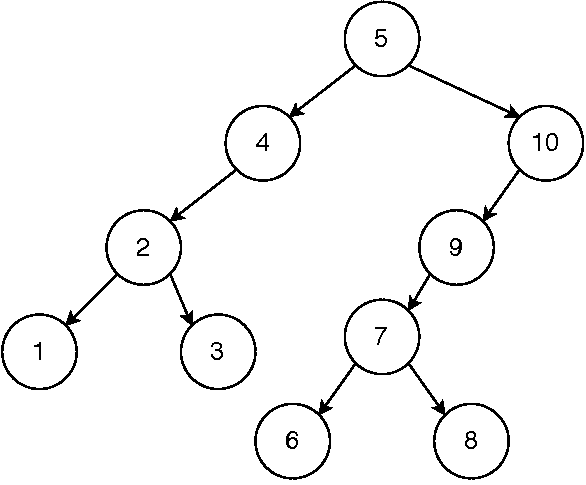
\includegraphics[scale=0.45]{img/splay-tree}
  \caption{从$[1, 2, ..., 10]$产生的伸展树。}
  \label{fig:splay-result}
\end{figure}

图\ref{fig:splay-result}给出了逐一插入$[1, 2, ..., 10]$的结果。伸展树产生了较平衡的结果。Okasaki发现了一条简单的伸展操作规则\cite{okasaki-book}:每次连续向左或者向右访问两次的时候,就旋转节点。当访问节点$x$的时候,如果连续向左侧或者右侧前进两次,我们将树$T$分割成两部分:$L$和$R$,其中$L$中的所有元素小于$x$,$R$中的元素都大于$x$。然后以$x$为根,$L$、$R$为左右子树构建一棵新树。分割过程递归地对子树进行伸展操作。

\be
\resizebox{\linewidth}{!}{\ensuremath{
\begin{array}{l}
\begin{array}{rcl}
partition\ \nil\ y & = & (\nil, \nil) \\
partition\ (L, x, R)\ y & = &  \\
\end{array} \\
\quad
\begin{cases}
  x < y & \begin{cases}
      R = \nil & (T, \nil) \\
      R = (L', x', R') & \begin{cases}
          x' < y & (((L, x, L'), x', A), B) \\
                  & \text{其中:}(A, B) = partition\ R'\ y \\
          \text{否则} & ((L, x, A), (B, x', R')) \\
                      & \text{其中:}(A, B) = partition\ L'\ y \\
        \end{cases} \\
    \end{cases} \\
  \text{否则} & \begin{cases}
      L = \nil & (\nil, T) \\
      L = (L', x', R') & \begin{cases}
         y < x' & (A, (L', x', (R', x, R))) \\
                 & \text{其中:}(A, B) = partition\ L'\ y \\
         \text{否则} & ((L', x', A), (B, x, R)) \\
                 & \text{其中:}(A, B) = partition\ R'\ y \\
      \end{cases} \\
    \end{cases}
  \end{cases} \\
\end{array}
}}
\ee

$partition$接受一棵树$T$和一个基准值$y$。如果树为空,结果为一对空的左右子树。否则,记树为$(L, x, R)$,我们比较基准值$y$和根节点的值$x$。如果$x < y$,分为两种子情况。(1)$R$为空,根据二叉搜索树的性质,所有的元素都小于$y$,结果为$(T, \nil)$。(2)否则,令$R = (L', x', R')$,若$x' < y$,我们递归地用基准值分割$R'$,将$R'$中所有小于$y$的元素放入树$A$,其余元素放入树$B$。结果为一对树,其中一棵为$((L, x, L'), x', A)$,另一棵为$B$。若$x' > y$,我们递归地用$y$分割$L'$得到结果$(A, B)$。最终的结果为一对树,一棵是$(L, x, A)$,另一棵是$(B, x', R')$。当$y < x$时,情况是对称的。

\index{伸展堆!插入}
我们可以用$partition$实现插入算法。当向一个伸展堆$T$插入一个新元素$k$时,我们先将堆分割为两棵子树$L$和$R$。其中$L$含有所有小于$k$的节点,而$R$含有剩余的部分。然后我们构建一棵新树,使用$k$作为根,$L$和$R$作为子树。

\be
insert\ T\ k = (L, k, R), \text{其中:} (L, R) = partition\ T\ k
\ee

\subsection{弹出顶部}
\index{伸展堆!top} \index{伸展堆!pop} \index{伸展堆!弹出}

由于伸展树本质上是二叉搜索树,最小的元素位于最左侧的节点。我们不断向左遍历以获取顶部元素。记非空的树为$T=(L, k, R)$,$top$函数可以定义如下:

\be
\begin{array}{rcl}
top\ (\nil, k, R) & = & k \\
top\ (L, k, R) & = & top\ L \\
\end{array}
\ee

这实际上就是二叉搜索树的$min$函数。弹出顶部时,需要将最小元素删除。同时每当连续向左访问两次,就执行一次伸展操作。

\be
\begin{array}{rcl}
pop\ (\nil, k, R) & = & R \\
pop\ ((\nil, k', R'), k, R) & = & (R', k, R) \\
pop\ ((L', k', R'), k, R) & = & (pop\ L', k', (R', k, R)) \\
\end{array}
\ee

第三条子式实际上执行了伸展操作,它并没有显式地调用$partition$函数,而是直接使用了二叉搜索树的性质。伸展树在平衡时堆顶操作的时间复杂度是$O(\lg n)$。

\subsection{合并}
\index{伸展堆!合并}

通过使用$partition$,我们可以实现$O(\lg n)$时间的合并算法。当合并两棵伸展树时,如果它们都不为空,我们可以将第一棵树的根节点作为新的根,然后将其作为基准值分割第二棵树。此后,我们递归地将第一棵树的子树合并。

\be
\begin{array}{rcl}
merge\ \nil\ T & = & T \\
merge\ (L, x, R)\ T & = & ((merge\ L\ L')\ x\ (merge\ R\ R')) \\
\end{array}
\ee

其中:

\[
  (L', R') = partition\ T\ x
\]

如果第一个堆为空,结果为另一个堆。否则,记第一个堆为$(L, x, R)$,用$x$为基准值分割$T$得到结果$(L', R')$,其中$L'$包含$T$中所有小于$x$的元素,而$R'$包含其余元素。接下来递归地将$L$和$L'$合并为新的左子树,将$R$和$R'$合并为右子树。

\section{小结}

本章中,我们介绍了通用的二叉堆概念。只要满足堆的性质,可以使用各种形式的二叉树来实现。用数组作为存储结构适于命令式实现,它将一棵完全二叉树映射为数组。方便进行随机访问。我们还介绍了直接用二叉树实现的堆,适于函数式实现。大部分操作的时间复杂度可以达到$O(\lg n)$,有些操作的分摊时间复杂度是$O(1)$的。Okasaki在\cite{okasaki-book}中给出了详细分析。一个自然的想法是将二叉树扩展到多叉树,这样就会得到其它数据结构如二项式堆、斐波那契堆和配对堆。参见第十章。

\begin{Exercise}
\Question{用命令式的方式实现左偏堆、斜堆、伸展堆。}
\end{Exercise}

\section{附录:例子程序}

在数组表示的完全二叉树中,利用位运算访问父节点和子树,索引从0开始:

\begin{lstlisting}[language = Bourbaki]
Int parent(Int i) = ((i + 1) >> 1) - 1

Int left(Int i) = (i << 1) + 1

Int right(Int i) = (i + 1) << 1
\end{lstlisting}

堆调整,将元素间的比较运算抽象为参数:

\begin{lstlisting}[language = Bourbaki]
void heapify([K] a, Int i, Less<K> lt) {
    Int l, r, m
    Int n = length(a)
    loop {
        m = i
        l = left(i)
        r = right(i)
        if l < n and lt(a[l], a[i]) then m = l
        if r < n and lt(a[r], a[m]) then m = r
        if m != i {
            swap(a, i, m);
            i = m
        } else {
            break
        }
    }
}
\end{lstlisting}

从数组构造堆:

\begin{lstlisting}[language = Bourbaki]
void buildHeap([K] a, Less<K> lt) {
    Int n = length(a)
    for Int i = (n-1) / 2 downto 0 {
        heapify(a, i, lt)
    }
}
\end{lstlisting}

弹出堆顶:

\begin{lstlisting}[language = Bourbaki]
K pop([K] a, Less<K> lt) {
    var n = length(a)
    t = a[n]
    swap(a, 0, n - 1)
    remove(a, n - 1)
    if a != [] then heapify(a, 0, lt)
    return t
}
\end{lstlisting}

寻找top-$k$:

\begin{lstlisting}[language = Bourbaki]
[K] topk([K] a, Int k, Less<K> lt) {
    buildHeap(a, lt)
    [K] r = []
    loop min(k, length(a)) {
        append(r, pop(a, lt))
    }
    return r
}
\end{lstlisting}

减小堆中某元素的值:

\begin{lstlisting}[language = Bourbaki]
void decreaseKey([K] a, Int i, K k, Less<K> lt) {
    if lt(k, a[i]) {
        a[i] = k
        heapFix(a, i, lt)
    }
}

void heapFix([K] a, Int i, Less<K> lt) {
    while i > 0 and lt(a[i], a[parent(i)]) {
        swap(a, i, parent(i))
        i = parent(i)
    }
}
\end{lstlisting}

堆插入:

\begin{lstlisting}[language = Bourbaki]
void push([K] a, K k, less<K> lt) {
    append(a, k)
    heapFix(a, length(a) - 1, lt)
}
\end{lstlisting}

堆排序:

\begin{lstlisting}[language = Bourbaki]
void heapSort([K] a, less<K> lt) {
    buildHeap(a, not . lt)
    n = length(a)
    while n > 1 {
        swap(a, 0, n - 1)
        n = n - 1
        heapify(a[0 .. (n - 1)], 0, not . lt)
    }
}
\end{lstlisting}

左偏堆合并:

\begin{Haskell}
merge E h = h
merge h E = h
merge h1@(Node _ x l r) h2@(Node _ y l' r') =
    if x < y then makeNode x l (merge r h2)
    else makeNode y l' (merge h1 r')

makeNode x a b = if rank a < rank b then Node (rank a + 1) x b a
                 else Node (rank b + 1) x a b
\end{Haskell}

斜堆合并:

\begin{Haskell}
merge E h = h
merge h E = h
merge h1@(Node x l r) h2@(Node y l' r') =
    if x < y then Node x (merge r h2) l
    else Node y (merge h1 r') l'
\end{Haskell}

伸展操作:

\begin{Haskell}
-- zig-zig
splay t@(Node (Node (Node a x b) p c) g d) y =
    if x == y then Node a x (Node b p (Node c g d)) else t
splay t@(Node a g (Node b p (Node c x d))) y =
    if x == y then Node (Node (Node a g b) p c) x d else t
-- zig-zag
splay t@(Node (Node a p (Node b x c)) g d) y =
    if x == y then Node (Node a p b) x (Node c g d) else t
splay t@(Node a g (Node (Node b x c) p d)) y =
    if x == y then Node (Node a g b) x (Node c p d) else t
-- zig
splay t@(Node (Node a x b) p c) y = if x == y then Node a x (Node b p c) else t
splay t@(Node a p (Node b x c)) y = if x == y then Node (Node a p b) x c else t
-- 否则
splay t _ = t
\end{Haskell}

伸展堆的插入:

\begin{Haskell}
insert E y = Node E y E
insert (Node l x r) y
    | x > y     = splay (Node (insert l y) x r) y
    | otherwise = splay (Node l x (insert r y)) y
\end{Haskell}

伸展树的分割:

\begin{Haskell}
partition E _ = (E, E)
partition t@(Node l x r) y
    | x < y =
        case r of
          E -> (t, E)
          Node l' x' r' ->
              if x' < y then
                  let (small, big) = partition r' y in
                  (Node (Node l x l') x' small, big)
              else
                  let (small, big) = partition l' y in
                  (Node l x small, Node big x' r')
    | otherwise =
        case l of
          E -> (E, t)
          Node l' x' r' ->
              if y < x' then
                  let (small, big) = partition l' y in
                  (small, Node l' x' (Node r' x r))
              else
                  let (small, big) = partition r' y in
                  (Node l' x' small, Node big x r)
\end{Haskell}

伸展树合并:

\begin{Haskell}
merge E t = t
merge (Node l x r) t = Node (merge l l') x (merge r r')
    where (l', r') = partition t x
\end{Haskell}

\ifx\wholebook\relax \else
\section{参考答案}
\shipoutAnswer

\begin{thebibliography}{99}

\bibitem{CLRS}
Thomas H. Cormen, Charles E. Leiserson, Ronald L. Rivest and Clifford Stein. ``Introduction to Algorithms, Second Edition''. The MIT Press, 2001. ISBN: 0262032937.(《算法导论》)

\bibitem{wiki-heap}
Heap (data structure), Wikipedia. \url{https://en.wikipedia.org/wiki/Heap_(data_structure)}

\bibitem{wiki-heapsort}
Heapsort, Wikipedia. \url{https://en.wikipedia.org/wiki/Heapsort}

\bibitem{okasaki-book}
Chris Okasaki. ``Purely Functional Data Structures''. Cambridge university press, (July 1, 1999), ISBN-13: 978-0521663502

\bibitem{rosetta-heapsort}
Sorting algorithms/Heapsort. Rosetta Code. \url{http://rosettacode.org/wiki/Sorting_algorithms/Heapsort}

\bibitem{wiki-leftist-tree}
Leftist Tree, Wikipedia. \url{https://en.wikipedia.org/wiki/Leftist_tree}

\bibitem{brono-book}
Bruno R. Preiss. Data Structures and Algorithms with Object-Oriented Design Patterns in Java. \url{http://www.brpreiss.com/books/opus5/index.html}

\bibitem{TAOCP-bheap}
Donald E. Knuth. ``The Art of Computer Programming. Volume 3: Sorting and Searching.''. Addison-Wesley Professional;
2nd Edition (October 15, 1998). ISBN-13: 978-0201485417. Section 5.2.3 and 6.2.3

\bibitem{wiki-skew-heap}
Skew heap, Wikipedia. \url{https://en.wikipedia.org/wiki/Skew_heap}

\bibitem{self-adjusting-heaps}
Sleator, Daniel Dominic; Jarjan, Robert Endre. ``Self-adjusting heaps'' SIAM Journal on Computing 15(1):52-69. doi:10.1137/0215004 ISSN 00975397 (1986)

\bibitem{wiki-splay-tree}
Splay tree, Wikipedia. \url{https://en.wikipedia.org/wiki/Splay_tree}

\bibitem{self-adjusting-trees}
Sleator, Daniel D.; Tarjan, Robert E. (1985), ``Self-Adjusting Binary Search Trees'', Journal of the ACM 32(3):652 - 686, doi: 10.1145/3828.3835

\bibitem{NIST}
NIST, ``binary heap''. \url{http://xw2k.nist.gov/dads//HTML/binaryheap.html}

\end{thebibliography}

\expandafter\enddocument
\fi
